\chapter{Introdução}

Este capítulo traz uma breve contextualização com o objetivo de justificar e construir um caminho lógico para a motivação da tese. Além disso, a declaração de tese é apresentada e a estrutura do documento é delineada.

\section{Contextualização}

Estimativas de recursos e reservas minerais demandam a construção de modelos numéricos de teores de longo prazo, que abrangem toda a extensão do depósito mineral e compreendem todo o tempo de vida da mina. Esses modelos são atualizados em intervalos de um a três anos de operação. Modelos de médio prazo podem ser construídos para planejar de um a seis meses no futuro do empreendimento. Enquanto modelos de curto prazo, são construídos com o objetivo de balizar, semanalmente ou diariamente, as decisões relativas a controle de teores e planejamento detalhado da mina.

Construir modelos numéricos de longo, médio e curto prazo para avaliação de recursos/reservas e planejamento de mina exige quatro grandes atividades \cite{rossi2013mineral}:

\begin{enumerate}[label=\roman*]
\item Coleta e gerenciamento de dados;
\item Interpretação e modelagem geológica;
\item Atribuição de teores;
\item Avaliação e gerenciamento da incerteza geológica e de teores.
\end{enumerate}

Após a coleta, gerenciamento e checagem dos dados, é necessário identificar diferentes domínios. A determinação dos domínios deve ser baseada no conhecimento geológico, i.e. zonas de oxidação, litologias, alteração ou limites estruturais e deve ser suportada por extensiva análise estatística (análise exploratória dos dados), incluindo análises variográficas. É importante que a definição dos domínios faça sentido espacial e geológico. Os domínios são, algumas vezes, baseados na combinação de duas ou mais variáveis para as quais a correlação entre os teores pode ser demonstrada. O procedimento pode ser bastante demorado, principalmente em depósitos multivariados, entretanto, as estimativas são melhoradas significativamente quando cuidadosamente limitadas por variáveis geológicas \cite{rossi2013mineral}. A \autoref{dom_def} mostra uma ilustração esquemática da definição dos domínios em um banco de dados.

\begin{figure}[H]
	\centering
	\caption{\label{dom_def}Ilustração esquematizando a definição dos domínios estacionários.}
	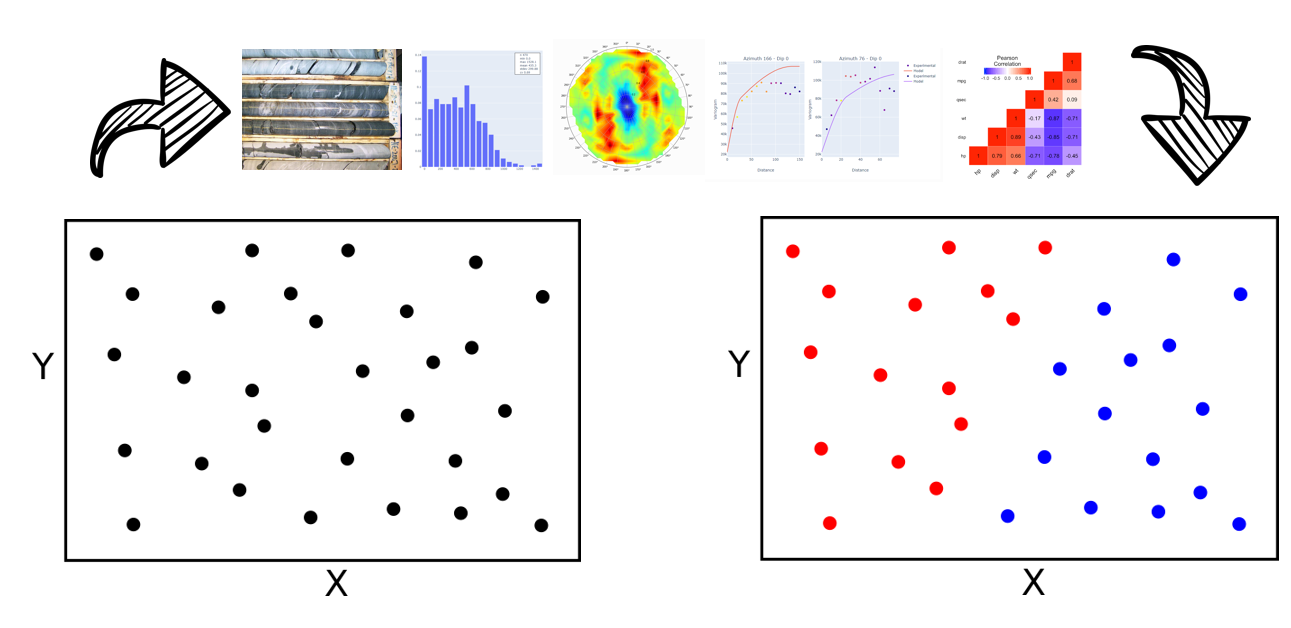
\includegraphics[width=0.8\textwidth]{capitulo_1/imagens/dom_def}
\end{figure}

A definição de diferentes domínios de estimativas, ou zonas estacionárias no interior do depósito, é necessária para a inferência geoestatística. Geralmente, o método usado na construção dos modelos numéricos de teores \cite{mclennanstationarity}. Isto é, os teores em cada domínio estacionário pertencem a populações estatísticas distintas, são caracterizados através de modelos de distribuição e de covariância específicos e devem ser modelados como funções aleatórias estacionárias diferentes. \cite{journel1978mining}. 

Uma função aleatória estacionária é uma representação probabilística de uma propriedade petrofísica com valor esperado e covariância constantes independente da localização \cite{mclennanstationarity}. Estacionariedade, definida por \citeonline{matheron1962traite}, é uma propriedade do modelo de função aleatória, não é uma característica intrínseca da variável. É uma decisão tomada pelo geomodelador e necessária para a inferência. Apesar dos domínios geológicos serem funções aleatórias estacionárias a tomada de decisão na sua determinação não necessariamente deve ser estritamente matemática. Podem ser consideradas propriedades geomecânicas, geometalúrgicas, petroquímicas, a geometria dentre outras. 

Os domínios estacionários não devem ser muito pequenos, dessa forma não incluiriam dados suficientes para descrição e inferência estatística confiável, e nem muito grandes, já que os dados, provavelmente, poderiam ser subdivididos em grupos geologicamente mais homogêneos. A definição adequada dos domínios estacionários é uma etapa importante na avaliação de recursos/reservas, a mistura de populações produz estimativas sub ótimas que superestimam ou subestimam teores e tonelagens. Além disso, nenhuma técnica geoestatística pode compensar uma definição de estacionariedade inadequada \cite{rossi2013mineral}.

Uma vez que os domínios estacionários tenham sido definidos, um modelo tridimensional com os limites de cada função aleatória estacionária deve ser construído: o modelo geológico. É necessário identificar a "jurisdição espacial"\ de cada função aleatória estacionária. A etapa de interpretação e modelagem geológica compreende a definição dos domínios estacionários e a criação do modelo geológico tridimensional que forma o alicerce para todo o trabalho de estimativa subsequente. Muitas vezes, o modelo geológico é o fator de maior importância na estimativas das tonelagens mineralizadas \cite{rossi2013mineral}. A \autoref{ilust_mpod} mostra uma ilustração esquemática do modelo geológico para o exemplo da \autoref{dom_def}.

\begin{figure}[H]
	\centering
	\caption{\label{ilust_mpod}Ilustração esquematizando a modelagem geológica.}
	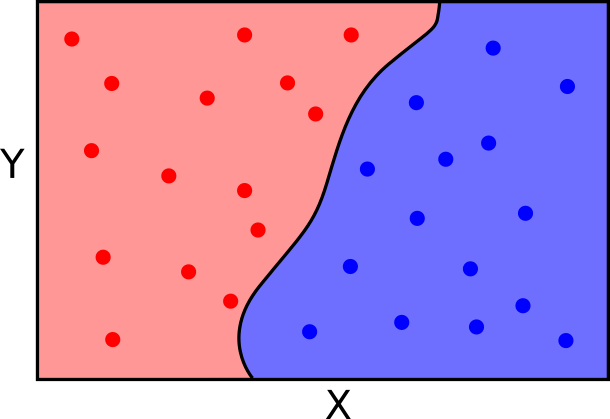
\includegraphics[width=0.6\textwidth]{capitulo_1/imagens/mapa_geomode_det}
\end{figure}

A abordagem tradicional para a criação de modelos geológicos tridimensionais é através da triangulação de polilinhas \footnote{Em computação gráfica: uma linha composta por vários segmentos, usada para compor imagens na tela \cite{oxfordonlinedictionary}.} (\textit{strings}) gerando sólidos que representam os corpos minerais. As polilinhas são digitalizadas manualmente em seções deslocadas, a partir dos dados de sondagem e conhecimento geológico prévio, por um geomodelador. As seções são unidas por linhas guias, que demarcam a conectividade entre as seções digitalizadas para triangulação adequada dos sólidos. Esse procedimento é referido como modelagem geológica explícita, já que os limites entre os diferentes domínios são definidos explicitamente por coordenadas (x,y,z) que posicionam a "colcha de retalhos"\ de triângulos \cite{mclennan2006boundsim,cowan2003practical}. A \autoref{explicitmodeling} ilustra a metodologia explícita para um típico depósito de veio.

\begin{figure}[H]
    \centering
	\caption{\label{explicitmodeling}Ilustração esquematizando a modelagem geológica explícita usando polilinhas e linhas guias.}
	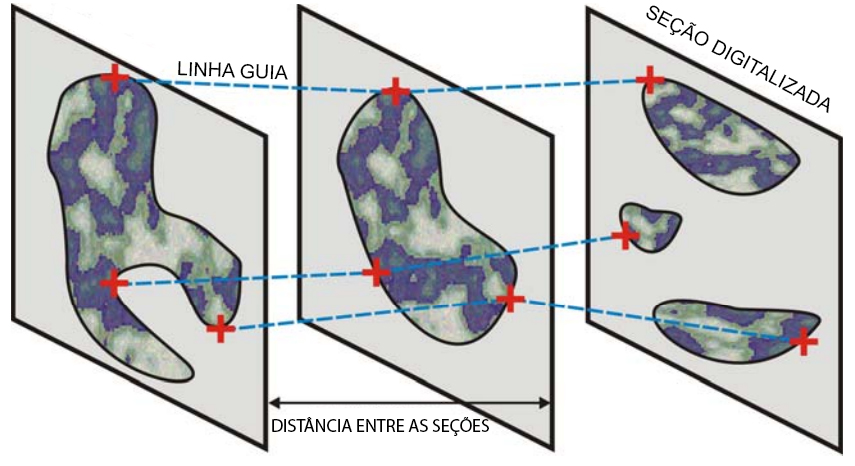
\includegraphics[width=0.8\textwidth]{capitulo_1/imagens/explicitmodeling}
	\legend{Modificado de \citeonline{mclennan2006boundsim}}
\end{figure}

De acordo com \citeonline{mclennan2006boundsim}, embora a metodologia seja direta e simples, principais motivos da sua ampla implementação na prática, e que \textit{softwares} modernos de mineração forneçam ferramentas computacionais para visualizar os dados de sondagem e agilizar o processo de digitalização \cite{silvaenhancedgeomodeling}, existem uma série de limitações e desvantagens. O processo é tedioso e demorado, digitalizar manualmente as polilinhas e uni-las por linhas guia, exige muito tempo de um profissional experiente. Em depósitos de alta complexidade, não é raro o geomodelador trabalhar até três meses no modelo geológico explícito. A geometria dos corpos geológicos muitas vezes precisa ser simplificadas para que o modelo seja concebido em tempo hábil. Por esse motivo, para a maioria das minas, apenas um modelo é construído e mantido, raramente há oportunidade de modelar interpretações geológicas alternativas e comparar estimativas de recursos baseadas em diferentes modelos \cite{cowan2003practical}.

Os modelos criados explicitamente são subjetivos e não replicáveis. O volume mineralizado é essencialmente composto por uma série de pequenas decisões subjetivas, já que cada ponto da polilinha em cada seção é escolhido por um geomodelador. Inevitavelmente, a "assinatura"\ do profissional é impressa nos limites dos domínios geológicos. Geomodeladores diferentes criam modelos diferentes a partir do mesmo banco de dados. Ademais, modelos explícitos são inflexíveis, é laborioso e demorado atualizar modelos explícitos a medida que novos dados são obtidos já que uma nova digitalização manual é necessária.

Embora a metodologia explícita seja demorada, laboriosa, subjetiva, não replicável, inflexível e que avaliar incertezas seja extremamente custoso, o limites entre domínios resultantes, geralmente, são realistas. Realismo geológico é um dos principais objetivos da modelagem e pode ser diretamente controlado durante o processo de digitalização.

\section{Motivação}

Em virtude da onerosidade em construir múltiplos modelos geológicos explícitos, é custoso avaliar a incerteza na localização dos limites dos diferentes domínios entre os dados amostrais, como mostrado na ilustração esquemática na \autoref{incerteza_limites}. Além da tediosa redigitalização manual de polilinhas e retriangulação, não existe forma direta de incorporar múltiplas realizações possíveis para a localização dos limites que representem a incerteza associada.

\begin{figure}[H]
    \centering
	\caption{\label{incerteza_limites}Ilustração esquemática destacando a incerteza na localização do limite entre os domínios azul e vermelho, entre os dados amostrais.}
	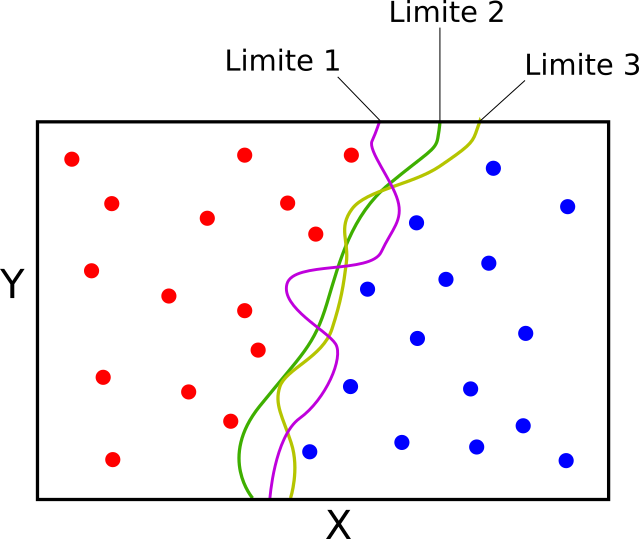
\includegraphics[width=0.6\textwidth]{capitulo_1/imagens/mapa_geomode_stoc}
\end{figure}

Em muitos casos, a incerteza do modelo geológico pode ser uma fonte de incerteza crucial. Em depósitos de veio de ouro, por exemplo, o volume mineralizado é um indicador econômico vital para o gerenciamento do projeto. Ignorar a incerteza volumétrica, considerando apenas um único modelo geológico explícito, pode ser ser devastador para o empreendimento. A incerteza associada ao modelo geológico deve ser avaliada.

Dadas as desvantagens do método explícito de modelagem geológica, pesquisas vêm sendo realizadas com o objetivo de automatizar, ou pelo menos, semi automatizar a modelagem e avaliar incerteza dos modelos geológicos.

Alguns dos métodos de simulação para variáveis categóricas, amplamente utilizados pela indústria da mineração, geram realizações que apresentam excessivo ruído. Além da necessidade de avaliar a incerteza dos modelos geológicos, existe também a preocupação de que os modelos finais apresentem limites contínuos e realistas entre as diferentes litologias do depósito. Não só para que os modelos tenham uma aparência mais agradável aos olhos, mas também para que a tarefa de definir \textit{diglines}, entre minério e estéril, seja facilitada e menos subjetiva.

\section{Declaração de tese}

\begin{tcolorbox}
A modelagem geológica implícita com funções distância assinaladas vem sendo utilizada há mais de uma década com sucesso como uma alternativa matemática à modelagem explícita na criação de modelos geológicos determinísticos. A metodologia está presente em diversos softwares comerciais de ampla utilização na indústria. Embora exista a necessidade de avaliar a incerteza associada ao modelo geológico, não há na literatura diferentes opções de métodos de avaliação de incerteza baseadas em funções distância assinaladas, especialmente para modelos multi-categóricos.
\end{tcolorbox}

\section{Objetivos}

O objetivo dessa tese é propor e investigar três diferentes metodologias para avaliação de incerteza em modelos geológicos   multi-categóricos usando funções distância assinaladas. As realizações obtidas a partir das metodologias propostas devem apresentar feições geológicas realistas e contínuas. Os métodos foram desenvolvidos e implementados em forma de \textit{plug-ins} para o \textit{software SGeMS/AR2GeMS} \cite{remy2009applied} ou \textit{jupyter notebooks} baseados em \textit{softwares} da biblioteca \textit{GSLib} \cite{deutsch1992geostatistical}.

\subsection{Desenvolvimento de software}

Foi desenvolvida uma \textit{suite} de \textit{plug-ins} de modelagem geológica para o \textit{software} geoestatístico \textit{SGeMS/AR2GeMS}: \href{https://github.com/robertorolo/LPM-Geomod_Suite}{LPM-Geomod-Suite}. Os \textit{plug-ins} abrangem todas as etapas da modelagem geológica com funções distância assinaladas e indicadores desde transformações, interpolação, e avaliação da incerteza associada ao modelo geológico. 

Um manual de instalação e uso dos \textit{plug-ins} é apresentado no \autoref{software}. 

\subsection{Avaliação de incerteza pela parametrização do suporte do \textit{kernel}}

É proposto um método para avaliação de incerteza baseado na parametrização do suporte do \textit{kernel}, que é a base para a interpolação das distâncias assinaladas utilizando funções de bases radiais (RBF). O \textit{kernel} é análogo ao variograma da krigagem. Para cada uma das variáveis, são geradas interpolações: para um cenário base, sem parametrização, um cenário otimista e um cenário pessimista. As diferentes propriedades interpoladas são combinadas para gerar diferentes realizações para o modelo geológico.  

\subsection{Avaliação de incerteza usando funções distância assinaladas e campos de probabilidade}

É proposto um método de avaliação de incerteza utilizando funções distância assinaladas e campos de probabilidade. Uma zona de incerteza é definida ao redor dos contatos, então, as distâncias assinaladas interpoladas no interior da zona de incerteza são transformadas em probabilidades. Em seguida, os campos de probabilidades gerados a partir de simulações Gaussianas não condicionais são utilizados para simular as diferentes realizações para o modelo geológico a partir do método de Monte Carlo.

\subsection{Simulação de contatos hierárquica para múltiplas categorias}

Uma adaptação do método proposto por \citeonline{wilde2012kriging} para múltiplas categorias simultâneas é proposto. Um algoritmo que identifica e define a frequência de ocorrência dos diferentes contatos é usado para agrupá-los de forma hierárquica. Os contatos representados por cada grupo são simulados de forma independente e a regra hierárquica é usada para construir as diferentes realizações do modelo geológico multi-categórico. 

\section{Estrutura da tese}

O capítulo 1 dessa tese traz uma introdução ao assunto modelagem geológica e avaliação de incerteza e apresenta: a motivação, declaração e objetivos da tese.

O capítulo 2 é uma revisão extensiva da literatura em modelagem geológica e avaliação de incerteza em modelos geológicos usando funções distância assinaladas. 

O capítulo 3 apresenta as metodologias propostas utilizando o conhecido \textit{dataset} \textit{Swiss Jura} \cite{goovaerts1997geostatistics} como prova de conceito em 2D. Um estudo de caso é conduzido para cada uma das metodologias propostas mostrando sua eficiência. As características e particularidades de cada uma delas e os resultados obtidos são discutidos.

Finalmente, o capítulo 4 apresenta as observações finais, um sumário das contribuições da tese e sugere trabalhos futuros.